\documentclass{article}

\usepackage{amssymb}
\usepackage[table,xcdraw]{xcolor}
\usepackage{amsmath}
\usepackage[brazilian]{babel}
\usepackage[utf8x]{inputenc}
\usepackage[sc]{mathpazo} 
\linespread{1.05}
\usepackage{microtype}
\usepackage[hang, small,labelfont=bf,up,textfont=it,up]{caption}
\usepackage{lettrine}
\usepackage{graphicx}
\usepackage{gnuplottex}
\usepackage{epstopdf}
\usepackage{multicol}
\usepackage{multirow}
\usepackage{array}
\usepackage{wrapfig}
\usepackage{svg}

\usepackage[hmarginratio=1:1,top=20mm,bottom=35mm,right=15mm,left=15mm,columnsep=20pt]{geometry}
%\usepackage{multicol} 
\usepackage{booktabs}
\usepackage{float} 
\usepackage{subfigure}
\usepackage{paralist} 
\usepackage{hyperref} 
\usepackage{abstract}
\renewcommand{\abstractnamefont}{\normalfont\bfseries}
\renewcommand{\abstracttextfont}{\normalfont\small\itshape}
\usepackage{titlesec}
\renewcommand\thesection{\Roman{section}}
\renewcommand\thesubsection{\Roman{subsection}} 
\titleformat{\section}[block]{\Large\scshape}{\thesection.}{1em}{} 
\titleformat{\subsection}[block]{\large}{\thesubsection.}{1em}{}
\usepackage{verbatim}
\usepackage{fancyhdr} 
\pagestyle{fancy} 
\fancyhead{} 
\fancyfoot{} 

\definecolor{cinzaclaro}{HTML}{84929f}

%AQUI VOCE COLOCA A SIGLA do grupo
\fancyhead[C]{Turma A $\cdot$ Física Experimental V $\cdot$ Bobinas de Helmholtz e Cálculo da Relação Carga/Massa do Elétron $\cdot$ Equipe 5}
\fancyfoot[C]{\thepage} \newenvironment{Figure}
  {\par\medskip\noindent\minipage{\linewidth}}
  {\endminipage\par\medskip}

% AQUI VOCÊ COLOCA O TÍTULO DO SEU EXPERIMENTO.

\title{\vspace{-18mm}\fontsize{16pt}{18pt}\selectfont\textbf{Bobinas de Helmholtz e Cálculo da Relação Carga/Massa do Elétron}} 


% AQUI VOCE COLOCA O NOME DOS AUTORES DO TRABALHO

\author{
\large
\textsc{Jonas Everton Gomes de Araújo\thanks{jonasega@discente.ufg.br }, Sérgio Wilson de Sá Roriz\thanks{sergiodx@discente.ufg.br}, Vinícius Martins Bento\thanks{vinicius\_martinsbento@discente.ufg.br}}\\[2mm]
\large Instituto de Física, Universidade Federal de Goiás \\
%\vspace{2mm}
\large Prof. \textsc{Ricardo Costa de Santana}
}
\date{}

\begin{document}
\maketitle

\thispagestyle{fancy} 
 
%___________________________________

\begin{abstract}
\textbf{Os fenômenos magnéticos são conhecido desde a antiguidade, mas fora a parir do século XIX com Oersted, que tal fenômeno começou a ser estudado em sua integralidade. De posse de duas bobinas de Helmholtz de 20 centímetros de raio, foram testados três arranjos, variando a distância entre as bobinas, 40 cm, 20 cm e 10 cm, com o intuito de obter um campo magnético uniforme entre elas no maior espaço possível. Os campos criados pelas bobinas foram medidos com um teslâmetro, variando a posição da ponta Hall a partir do centro geométrico primeiramente na direção axial e em seguida na direção radial. Encontrado o melhor arranjo, um tubo de raios catódicos foi instalado na região de campo magnético uniforme. Quando alimentado por uma ddp, o tubo emite um feixe de elétrons que ao colidir com átomos do gás no interior do tubo os faz emitir luz, o que permite  a visualização do feixe de elétrons. Quando uma corrente elétrica percorre as bobinas, o campo magnético uniforme criado na região entre elas faz com que o feixe de elétrons seja defletido pois a força magnética atua como força centrípeta. Ao medir a ddp que acelera o feixe, a corrente que cria o campo magnético e o raio da curva que o feixe de elétrons perfaz, calcula-se a relação entre a carga elétrica do elétron e sua massa.}
\end{abstract}
%
\vspace{0.5cm}

\setlength{\columnsep}{10pt}%
\section{Introdução}

Em determinados casos, é necessário produzir um campo magnético uniforme de baixa intensidade em um volume relativamente grande. Para tal fim, é, em geral, utilizado o equipamento desenvolvido por Hermann Ludwig Ferdinand von Helmholtz (1821-1894), denominado atualmente por \textbf{bobina de Helmholtz}. Esse aparelho consiste de duas bobinas coaxiais circulares separadas por uma distância escolhida cada uma contendo um número $N$ de espiras de raio $R$ com correntes fluindo no mesmo sentido. Veja figura \ref{helmholtz}.

\begin{wrapfigure}[14]{r}{0.4\textwidth}
    \centering
    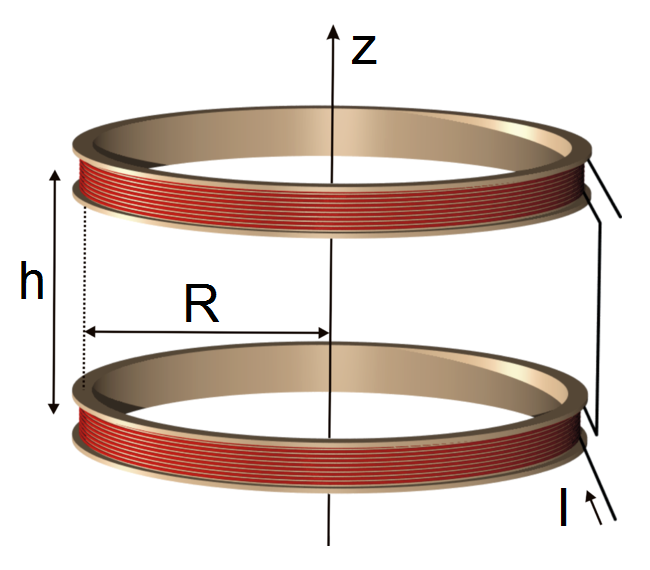
\includegraphics[width=7cm]{./Imagens/Helmholtz.png}
    \caption{Esquematização de uma bobina de Helmholtz. }
    \label{helmholtz}
\end{wrapfigure}

As aplicações da bobina de Helmholtz são várias, por exemplo: determinação das componentes vertical e horizontal do campo magnético terrestre, bem como sua anulação em determinado volume; calibração de medidores de campo magnético de baixa frequência; estudo dos efeitos de campos magnéticos em componentes ou equipamentos eletrônicos; medidas de susceptibilidade magnética; calibração de equipamentos de navegação; estudo de efeitos biomagnéticos; ajuste de tubos de raios catódicos; estudo da performance de tubos de fotomultiplicadoras em campos magnéticos; medidas de magnetorresistência; desmagnetização de pequenas peças de materiais ferromagnéticos usados na ciência de naves espaciais. Nesse experimento, ela foi usada para a determinação da carga específica do elétron.

Para entender o funcionamento de uma bobina de Helmholtz, deve-se lembrar que o campo magnético formado por uma bobina circular é dado por:

\begin{equation}
    \label{biotsavartequation}
    d \vec B =  \frac{\mu _0 I}{4 \pi} \frac{d \vec l \times \vec \rho} {\rho ^3}
\end{equation}
\begin{wrapfigure}[15]{r}{0.4\textwidth}
    \centering
    \includesvg[width=7.4cm]{./Imagens/SpireCourant.svg}
    \caption{Esquema demonstrando a direção e sentido dos vetores presentes na Lei de Biot-Savart (eq. \ref{biotsavartequation}). }
    \label{biotsvartimage}
\end{wrapfigure}
onde $\mu _0$ é permeabilidade magnética do vácuo, $\vec \rho$ é o vetor que vai do elemento condutor $d \vec l$ até ponto de de medida $\vec B$, e $d \vec B$ é perpendicular ao vetores $\vec \rho$ e $d \vec l$. Veja a figura \ref{biotsvartimage}.

Como o vetor $d \vec l$ é perpendicular aos vetores $\vec \rho$ e $d \vec B$ e ainda perpendicular ao plano da figura, enquanto os outros dois vetores estão no plano da figura, a equação \ref{biotsavartequation} pode ser reescrita como:

\begin{equation}
    dB = \frac{\mu _0 I}{4 \pi} dl = \frac{I}{4 \pi} \frac{\mu _0 dl}{R^2 +z^2}
\end{equation}

sendo $z$ a distância do centro da espira ao ponto onde estamos calculando o campo. Como mostrado na figura, $dB$ pode ser dividido em duas componentes, uma radial $dB$ e uma axial $dB _z$ . Para qualquer elemento $dl$ que escolhermos na espira a componente $dB _z$ do campo terá sempre a mesma direção, podendo, portanto serem somadas, já as componentes $dB _r$ se anulam aos pares. Sendo assim o campo na direção radial é nulo, ou seja, $\mathbf{B _r = 0}$ e o campo ao longo da direção $z$ (axial) é dado por:

\begin{equation}
    \label{bz}
    B _z = \frac{\mu _0 I}{2}\frac{R^2}{(R^2 + z^2)^{\frac{3}{2}}} =  \frac{\mu _0 I}{2R}\frac{1}{(1 + (z/R)^2)^{\frac{3}{2}}}
\end{equation}

O campo magnético de uma bobina circular de $N$ espiras é então obtido multiplicando-se o número de espiras pela equação (\ref{bz}). Dessa forma, o campo ao longo do eixo das duas bobinas idênticas a uma distância a do centro das bobinas é:

\begin{equation}
    B(z,r=0) =  \frac{\mu _0 I N}{2R} \left [ \frac{1}{(1 + A^2)^{\frac{3}{2}}} + \frac{1}{(1 + A'^2)^{\frac{3}{2}}} \right ]
\end{equation}
Com
\begin{equation*}
    A = \frac{z-a/2}{R} \qquad e \qquad A' = \frac{z+a/2}{R}     
\end{equation*}

Quando  $z = 0$, o campo magnético tem um valor máximo para $a < R$ e mínimo para $a > R$. A dependência de $B$ com a posição ao longo do eixo axial das bobinas é virtualmente uniforme para o intervalo $\frac{-R}{2} < z < \frac{R}{2}$, quando $a = 0$. O campo $B$ no ponto médio entre as bobinas quando a separação a entre elas for igual ao raio $R$ é:

\begin{equation}
    B(0,0) = \frac{\mu _0 I N }{2R} \frac{2}{(5/4)^{\frac{3}{2}}} = 0,716 \mu _0 N \frac{I}{R}
\end{equation}
onde escolhemos como origem do sistema de coordenadas o ponto médio entre as bobinas sobre o eixo axial, para uma bobina com N = 154 espiras, raio R = 20 cm e corrente I = 4,0 A, o valor do campo B é de:

\begin{equation}
    B(0,0) = 2,77 \ mT
\end{equation}

Em 1897, Joseoh John Thomson(1856-1940) calculou a relação entre a carga elétrica e a massa do elétron, usando como aparato a bobina de Helmholtz. Esses experimento lhe valeu o Prêmio Nobel da Física, em 1906. Para isso, Thomson usou uma ideia simples: se um portador de carga elétrica estiver se movendo em um campo magnético perpendicular à sua velocidade, então o portador de carga sofrerá uma deflexão em sua trajetória.

A força magnética $\vec F$  que age sobre um portador de carga que se movimenta com velocidade $\vec v$ num campo magnético $\vec B$ é dada pela relação vetorial apresentado abaixo:

\begin{equation}
    \vec F  = q \cdot ( \vec v \times \vec B)
\end{equation}

Se o feixe de elétrons é perpendicular ao campo magnético gerado pelas bobinas, então a Força de Lorentz apresentado acima se reduz à da equação a seguir, que também mostra como fica estabelecida a velocidade do portador de carga quando a Força Magnética atua como Força Centrípeta no feixe de elétrons:

\section{Descrição experimental}


O experimento executado em laboratório divide-se em duas partes: na primeira parte são realizadas repetidas medições do número de decaimentos registrados no decorrer de um minuto. Na segunda parte é medida a atenuação na detecção da radiação em função da distância e em função da espessura de material posicionado entre a fonte e o detector.

\subsection{Primeira Etapa}

Para a primeira parte, utiliza-se uma capela contendo uma fonte radioativa emissora de raios gama em que há instalado um detector Geiger já posicionado a determinada distância da fonte (de acordo com o roteiro adotado, presume-se que deva ser a distância em que a taxa média é de 200 contagens por minuto). Veja figura .

O detector também controla o tempo de detecção; ele é programado para executar a detecção durante um minuto, de modo que não serão consideradas aqui as incertezas decorrentes da medição do intervalo de tempo, o que simplifica bastante o cálculo de propagação de incertezas.

Com esse aparato, foram realizados 100 medições (eventos) de contagem de decaimentos da amostra de Cobalto-60.

\subsection{Segunda Etapa}

Para a segunda parte, inicialmente é medida a radiação de fundo, o que é feito deixando o medidor Geiger detectar por dez minutos longe de qualquer fonte radioativa. Qualquer decaimento registrado será devido ao ambiente, e não à fonte radioativa a ser estudada. Novamente não será considerada a incerteza advinda da medição do tempo.

Em seguida, são utilizados suportes de chumbo em um dos quais é posicionado um bastão contendo uma amostra de Cobalto-60 e em outro a ponta do detector Geiger.

\newpage

\begin{wrapfigure}{r}{0.4\textwidth}
    \centering
    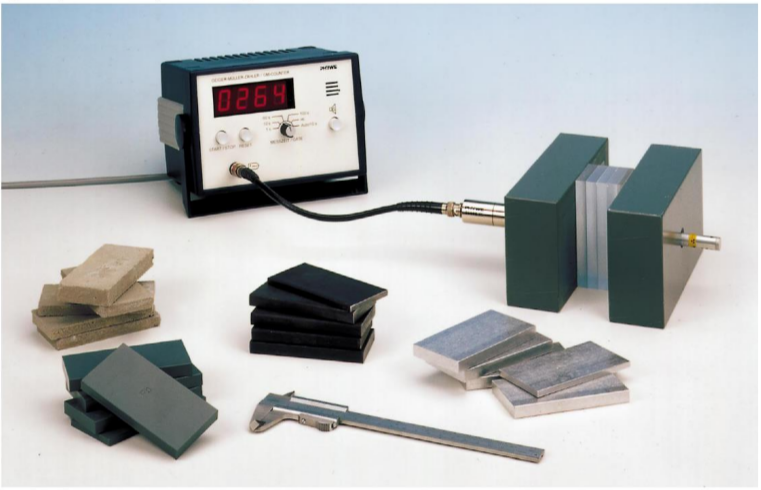
\includegraphics[width=7cm]{2etapa.png}
    \caption{Aparato experimental da segunda etapa.}
    \label{2etapa}
\end{wrapfigure}

Os dois suportes são alinhados e, com o auxílio de uma régua de acrílico, faz-se deslizar um dos suportes perpendicularmente à régua de modo a medir a distância entre a fonte e o detector, a fim de avaliar a atenuação da detecção à medida que essa distância aumenta. As medições são feitas durante dois minutos para cada uma das 14 distâncias consideradas, que variam de 3 cm a 16 cm.

Em seguida posicionam-se placas de diferentes materiais entre a fonte e o detector de modo a variar a espessura do material interveniente, executando assim 7 medições para cada material, cuja espessura variou de 1 mm a 30 mm. Cada uma dessas medições durou 3 minutos, e foram utilizados dois materiais diferentes: acrílico e chumbo.

\section{Resultados e Discussão}

\subsection{Primeira Etapa}

Seguindo o procedimento experimental foram feitas medições para as grandezas descritas em cada uma das etapas. Na tabela \ref{tabela_1}  são apresentados os resultados das 100 medições das contagens de emissões de raios gama oriundas da amostra utilizada em laboratório. 

\begin{table}[ht]
    \centering
    \begin{tabular}{|c|c|c|c|c|c|c|c|}
    \hline
    \rowcolor{cinzaclaro}
~ \textbf{Evento} ~ & \textbf{Contagem}& ~ \textbf{Evento} ~ & \textbf{Contagem} & ~ \textbf{Evento} ~ & \textbf{Contagem} & ~ \textbf{Evento} ~ & \textbf{Contagem} \\ \hline
1 & 185 & 26 & 163 & 51 & 211 & 76 & 187 \\ \hline
2 & 195 & 27 & 189 & 52 & 226 & 77 & 168 \\ \hline
3 & 184 & 28 & 199 & 53 & 200 & 78 & 186 \\ \hline
4 & 175 & 29 & 196 & 54 & 203 & 79 & 220 \\ \hline
5 & 165 & 30 & 183 & 55 & 218 & 80 & 177 \\ \hline
6 & 190 & 31 & 194 & 56 & 207 & 81 & 186 \\ \hline
7 & 170 & 32 & 221 & 57 & 221 & 82 & 223 \\ \hline
8 & 223 & 33 & 220 & 58 & 212 & 83 & 165 \\ \hline
9 & 187 & 34 & 219 & 59 & 164 & 84 & 183 \\ \hline
10 & 179 & 35 & 219 & 60 & 202 & 85 & 183 \\ \hline
11 & 166 & 36 & 169 & 61 & 220 & 86 & 228 \\ \hline
12 & 209 & 37 & 227 & 62 & 177 & 87 & 230 \\ \hline
13 & 170 & 38 & 172 & 63 & 198 & 88 & 222 \\ \hline
14 & 214 & 39 & 183 & 64 & 217 & 89 & 185 \\ \hline
15 & 171 & 40 & 163 & 65 & 224 & 90 & 189 \\ \hline
16 & 190 & 41 & 229 & 66 & 160 & 91 & 218 \\ \hline
17 & 186 & 42 & 181 & 67 & 200 & 92 & 194 \\ \hline
18 & 192 & 43 & 168 & 68 & 191 & 93 & 173 \\ \hline
19 & 209 & 44 & 166 & 69 & 162 & 94 & 173 \\ \hline
20 & 211 & 45 & 219 & 70 & 204 & 95 & 182 \\ \hline
21 & 181 & 46 & 220 & 71 & 208 & 96 & 229 \\ \hline
22 & 211 & 47 & 172 & 72 & 162 & 97 & 169 \\ \hline
23 & 223 & 48 & 174 & 73 & 190 & 98 & 177 \\ \hline
24 & 219 & 49 & 194 & 74 & 191 & 99 & 226 \\ \hline
25 & 182 & 50 & 215 & 75 & 181 & 100 & 191 \\ \hline
    \end{tabular}
\caption{Medidas com tempo de contagem fixo de um minuto.}
    \label{tabela_1}
\end{table}

Com os dados obtidos, foi calculada a média acumulada \cite{fisicaexpV} da taxa de contagem, que é dada pela equação \ref{media_acum_equation}, onde $j$ é o numero total de medições e $t _i$ o tempo associado a obtenção de contagens da medição $i$.

\begin{equation}
\label{media_acum_equation}
r_i (j) = \frac{\sum _{i=1} ^{j} c_i}{\sum _{i=1} ^{j} t_i}
\end{equation}
O gráfico da média acumulada como função do número sequencial $j$ da contagem pode ser visto na Figura \ref{media_acum}, observa-se que a média acumulada converge para uma contagem de, aproximadamente, \textbf{194,55}.

\begin{figure}[H]
    \centering
    \begin{gnuplot}[terminal = epslatex, terminaloptions = color, terminaloptions = {size 18.5cm,10.5cm}]
    set notitle
    set xlabel "Medição j"
    set ylabel "Média acumulada $r(j)$"
    set key right bmargin
    set style line 1 lc rgb "#3a3a3a" lt 0 lw 1
    set style line 2 lc rgb "#3a3a3a" lt 0 lw 1
    set grid xtics ytics mxtics mytics ls 1, ls 2
    set mxtics 3
    set mytics 2
    set xr [0:101]
    set yr [180:200]
    set samples 300
    plot "./Dados/media_acum.txt" u 1:2 notitle pt 7 ps 1.5 w lp
    \end{gnuplot}
    \caption{Média acumulada da taxa de contagem $j$ em função do número sequencial do evento. O código para gerar esses pontos encontram-se no GitHub. \href{https://github.com/Vento09/Fisica\_exp\_V}{Clique aqui para acessar.}}
    \label{media_acum}
\end{figure}
Pelo gráfico apresentado acima na figura \ref{media_acum}, percebemos que à medida que acumulamos mais eventos de contagem, mais bem definida torna-se a taxa média, isto é, mais o processo aleatório de decaimento radioativo aproxima-se de um processo “estacionário”, que ocorre a uma taxa média bem definida.

Efetuou-se então o teste do $\chi ^2$ para as primeiras 81 contagens obtidas. A definição desse teste, conforme o roteiro seguido \cite{fisicaexpV} é apresentado na equação \ref{chi2} abaixo, em que $r _i$ é a i-ésima taxa de contagem, além de $m = 194$ ser a média das primeiras 81 contagens.
\begin{equation}
   \label{chi2}
	\chi ^2 = \sum_{i=1} ^{81}\frac{(r_i - m)^2}{m}
\end{equation}Ainda, de acordo, com o roteiro, um valor para $\chi ^2$ entre 64,3 e 96,6 indica funcionamento satisfatório do sistema de detecção, o que não ocorreu com os dados utilizados dando o resultado \ref{chi2resultado} abaixo:
\begin{equation}
	\label{chi2resultado}
	\chi ^2 = 170,01
\end{equation}Em seguida, foi calculado o desvio padrão ($\sigma$). Para isso, foi utilizado a equação \ref{desvio_padrao} abaixo, seguido com seu resultado, usando $m = 195$ que é a média das $n = 100$ contagens.

\begin{equation}
	\label{desvio_padrao}
    \sigma = \sqrt{\frac{\sum _{i=1} ^{n} (c_i -m)^2}{(n-1)}} = 20,84
\end{equation}
E também, calculou-se o desvio médio ($\delta _m$). Para isso, foi utilizado a equação abaixo, seguido com seu resultado, usando $m =195$ que é a média das $n=100$ contagens.
\begin{equation}
	\delta _m = \frac{\sum _{i=1} ^{n} |c _i - m|}{n} = 18,10
\end{equation}
O parâmetro $\mu$ da Distribuição de Poisson, mostrado na equação  é o valor médio das medições e, segundo John R. Taylor , em tradução livre, “a distribuição de Poisson com contagem média tem desvio padrão.” (TAYLOR. p.249)\cite{taylor}. A FIGURA 7 a seguir traz os resultados de $\mu$ e de $\sqrt{\mu}$ calculados com os dados medidos em laboratório:

\begin{equation}
	m(100) = 194,55 \Rightarrow \sqrt{m(100)} = 13,94 \therefore \mu = 195 \pm 14 \ cpm
\end{equation}
É interessante também efetuar o teste do $\chi ^2$ definido de outra forma: supõe-se que para muitas medições seria possível usar a aproximação gaussiana. Define-se então quatro intervalos a partir da média e do valor de um desvio, a saber, são definidos os intervalos $I_1: v < 181$, $I_2 : 181 < v < 195$, $I _3 : 195 < v < 209$, $I_4 : v > 209$ e enumera-se dentre as contagens quantas pertencem a quais desses quatro intervalos. De posse dessas quantidades, compara-se as quantidades observadas em cada intervalo $O_I$ com as quantidades esperadas $E_I$, que são definidas pelo produto do número total de medições pela probabilidade gaussiana de um resultado qualquer situar-se em cada um dos quatro intervalos, isto é, a um ou a dois desvios da média (68\% ou 32\%, respectivamente divididas em dois intervalos cada). As contagens que eventualmente se situam na fronteira entre dois intervalos contam pela metade em cada intervalo fronteiriço (TAYLOR. p.266)\cite{taylor}. Essa classificação dos dados obtidos é mostrada na tabela abaixo:

\begin{table}[hb!]
    \centering
    \begin{tabular}{|c|c|c|c|}
    \hline
    \rowcolor{cinzaclaro}
\textbf{Intervalo} & ~ ~ \textbf{Qtde. observadas} ~ ~   & \textbf{Qtde. esperadas}  & ~ ~ \textbf{Diferença $\mathbf{O _i - E _i}$} ~ ~  \\ \hline
$\qquad \qquad \qquad \quad \ \ \ v < \mu - \sqrt{\mu} = 181 $     & 28,5         & 16    & 12,5         \\ \hline
$181 =\mu - \sqrt{\mu} < v < \ \quad \mu \ \quad = 195$     & 28         & 34     & -6         \\ \hline
$195 =  \ \quad \mu \quad \  < v < \mu + \sqrt{\mu} =209$     & 11,5         & 34     & 22,5         \\ \hline
$209 = \mu + \sqrt{\mu} < v \ \ \quad \qquad \qquad \qquad $      & 32          & 16     & 16         \\ \hline
    \end{tabular}
    \caption{Caption}
    \label{tabelachi2}
\end{table}

Usando essas definições e os dados da tabela \ref{tabelachi2}, a equação que se segue apresenta a definição do teste do $\chi ^2$ e o resultado obtido com as $n= 100$ contagens submetidas ao teste:

\begin{equation}
    \chi ^2 = \sum _{I=1} ^{4} \frac{(O _I - E_I)^2}{E _I} = 41,71
\end{equation}Como o valor de $\chi ^2$  muito maior que 4, pode-se inferir que os dados não são satisfatórios para aproximar-se a uma gaussiana e que é demonstrado no gráfico. Com os dados da tabela \ref{tabelachi2}, nota-se que apenas as contagens que se situam no segundo intervalo, que abrange as contagens entre 181 e 195, parece estar próximo de uma distribuição gaussiana. Os demais intervalos não se aproximam das porcentagens esperadas.

Para a visualização da frequência de ocorrência das contagens, foi feito um histograma (Figura \ref{grafico_poisson}) com 15 intervalos entre 160 a 230. Cada intervalo com o agrupamento de 5 medições. No mesmo gráfico, também foram colocadas as frequências de ocorrência da distribuição de Poisson. Comparando as medições, observa-se que o comportamento dos dados experimentais se comportam de forma totalmente diferente aos teóricos.

\begin{figure}[H] %n B cte
    \centering
    \begin{gnuplot}[terminal = epslatex, terminaloptions = color, terminaloptions = {size 18.5cm,9.5cm}]
    set notitle
    set xtics ("160-164" 0, "165-169" 1,"170-174" 2, "175-179" 3, "180-184" 4, "185-189" 5,"190-194" 6, "195-199" 7, "200-204" 8, "205-209" 9, "210-214" 10, "215-219" 11, "220-224" 12, "225-229" 13, "230-234" 14) rotate by -45
    set xlabel "Contagens"
    set ylabel "Frequência (em porcentagem)"
    set style histogram clustered gap 1 title textcolor lt 0
    set style fill solid 1.00 border lt 1
    set style line 1 lc rgb "#3a3a3a" lt 0 lw 1
    set style line 2 lc rgb "#3a3a3a" lt 0 lw 1
    set grid xtics ytics mxtics mytics ls 1, ls 2
    set mxtics 1
    set mytics 1
    set xr [-0.5:14.5]
    set yr [0:40.8]
    set samples 300
    plot "./Dados/poisson.txt" u 2 title "Experimental" w histogram,  "./Dados/poisson.txt" u 1 title "Poisson" smooth csplines lw 5
    \end{gnuplot}
    \caption{Histogramas acoplados das frequências de ocorrência da distribuição experimental e da distribuição de Poisson.}
    \label{grafico_poisson}
\end{figure}

\subsection{Segunda Etapa}

\begin{wraptable}[26]{r}{0.3\textwidth}
    \centering
    \begin{tabular}{|c|c|c|}
    \hline
    \rowcolor{cinzaclaro}
\textbf{r(cm)} & {$\mathbf{\dot N'(r)}$} & {$\mathbf{\dot N(r)}$}  \\ \hline
3     & 162     & 62,2  \\ \hline 
4     & 127     & 44,7  \\ \hline 
5     & 100     & 31,2   \\ \hline 
6     & 78      & 20,2  \\ \hline 
7     & 69      & 15,7   \\ \hline 
8     & 59      & 10,7   \\ \hline 
9     & 51      & 6,7   \\ \hline
10     & 45     & 3,7   \\ \hline
11     & 47     & 4,7   \\ \hline
12     & 40     & 1,2   \\ \hline
13     & 37     & -   \\ \hline
14     & 35     & -   \\ \hline
15     & 31     & -   \\ \hline
16     & 29     & -    \\ \hline
    \end{tabular}
	\caption{Na primeira coluna, apresenta a distância r, na segunda contagem de radiação gama $\gamma$ durante 2 min e na terceira a contagem efetiva por minuto}
    \label{tabela_2min}
\end{wraptable}

O primeiro passo foi medir a radiação de fundo da sala durante 10 minutos. O contador Geiger-Müller realizou 188 contagens nesse tempo, logo o valor por minuto da intensidade de radiação é dado por:

\begin{equation}
    \label{radiacaofundo}
    \frac{\dot N}{1 \ min} =\dot N _0 =\frac{188}{10 \ min} = 18,8 \ contagens/min
\end{equation}

Posteriormente, foram feitas contagens de radiação em função da distância $r$ $\dot N'(r)$ como mostra a tabela \ref{tabela_2min} ao lado direito. Para obter a taxa de contagem das intensidades efetivas, foram utilizadas a Equação (\ref{eq_sem_abs}) 

\begin{equation}
    \label{eq_sem_abs}
    \dot N(r) = \dot N'(r) - \dot N _0
\end{equation}

Os valores da contagem foram dividas pelo tempo (2 minutos) e, em seguida, diminuídas pelo valor da radiação de fundo $\dot N _0$ encontrado na equação acima (\ref{radiacaofundo}) e que podemos ver seus resultados na terceira coluna da tabela \ref{tabela_2min}.  Para os dados, de distância $r = 13 \ cm$ até a distância $r = 16 \ cm$, houve uma contagem por minuto $\dot N'(r)$ menor do que a radiação de fundo $N _0$. Por isso, foram ignorados já que não faz sentido a fonte de radiação diminuir a quantidade detectada.

Essa taxa de contagem $\dot N(r)$, tem uma relação exponencial com a distância $r$ que pode ser obtida através da Equação (\ref{N_arb}):


\begin{equation}
    \label{N_arb}
    \dot N(r) = ar^b
\end{equation}

\begin{wraptable}[15]{r}{0.3\textwidth}
    \centering
    \begin{tabular}{|c|c|c|}
    \hline
    \cellcolor{cinzaclaro}\textbf{Material} & \cellcolor{cinzaclaro}\textbf{Acrílico} & \cellcolor{cinzaclaro}\textbf{Chumbo} \\ \hline
\cellcolor[HTML]{CFCFCF}\textbf{d(cm)} & \cellcolor[HTML]{CFCFCF}~ ~ \textbf{N} ~ ~  & \cellcolor[HTML]{CFCFCF}~ {$\mathbf{\dot N'(r)}$}  ~  \\ \hline
1     & 219         & 127         \\ \hline
5     & 206         & 112         \\ \hline
10   & 202          & 103         \\ \hline
15    & 178         & 105         \\ \hline
20    & 139         & 100         \\ \hline
25    & 134         & 99          \\ \hline
30    & 125         & 80          \\ \hline
    \end{tabular}
    \caption{Contagem de radiação gama $\gamma$ durante 3 min em função da espessura x(cm) do Acrílico e do Chumbo }
    \label{tabela_absorvedor}
\end{wraptable}

Se aplicarmos logaritmo dos dois lados, obteremos uma equação linear sendo $b$ o valor da inclinação, $y=log(\dot N(r))$ e $ x = log(r)$ 
\begin{equation}
	log (\dot N(r)) = log(a) + b \cdot log(r)
\end{equation}
E de acordo com fabricante \cite{fisicaexpV}, devemos obter o valor de $b = (-2,07 \pm 0,01$)

O gráfico log-log pode ser visto na figura \ref{sem_abs} onde foi encontrado um $b = (2,592 \pm 0,24)$ que é próximo ao dado do fornecedor.

Em seguida, foi realizado contagens de radiação em função da espessura $\dot N(d)$ dos materiais de Acrílico e do Chumbo como mostra a tabela \ref{tabela_absorvedor}. Esses dois materiais foram utilizados como absorvedores e para o cálculo da contagem efetiva $\dot N(d)$ foi utilizado a equação \ref{eq_com_abs}

\begin{equation}
    \label{eq_com_abs}
    \dot N(d) = \dot N'(d) - \dot N _0
\end{equation}

\begin{figure}[H] %p B cte
    \centering
    \begin{gnuplot}[terminal = epslatex, terminaloptions = color, terminaloptions = {size 18.5cm,8cm}]
    set notitle
    set xlabel "log($r$)"
    set ylabel "log($N(r)$)"
    set key right bmargin
    set style line 1 lc rgb "#3a3a3a" lt 0 lw 1
    set style line 2 lc rgb "#3a3a3a" lt 0 lw 1
    set grid xtics ytics mxtics mytics ls 1, ls 2
    set mxtics 3
    set mytics 2
    set xr [0.46:1.1]
    set yr [0:2.1]
    set samples 300
    plot "./Dados/sem_abs.txt" u 1:2 notitle pt 7 ps 1.5, -2.592063758*x + 3.238220754 notitle
    \end{gnuplot}
    \caption{Média acumulada da taxa de contagem $j$ em função do número sequencial do evento.}
    \label{sem_abs}
\end{figure}

A atenuação dos raios gama quando passam por um absorvedor de espessura $d$ é dada pela Equação (\ref{atenuacao}):

\begin{equation}
    \label{atenuacao}
    \dot N(d) = \dot N(0)e^{-\mu d}
\end{equation}

Onde $\dot N(d)$ é a contagem depois da atenuação sofrida pelo meio e $\dot N(0)$ é a intensidade de radiação quando não há absorção. Aplicando um ajuste linear do tipo

\begin{equation}
    \label{semcriatividade}
    \dot N(d) = ae^{bd}
\end{equation}
para cada um dos materiais e comparando as Equações (\ref{atenuacao}) e (\ref{semcriatividade}) temos que $\mu = −b$, assim para o Acrílico, obtivemos $\mu = (0,021 \pm 0,0022) cm ^{−1}$ e para o Chumbo, $\mu = (0,012 \pm 0,0017) cm ^{−1}$ . Os valores dados pelo fornecedor são $\mu = 0,078 cm ^{−1}$ para o Acrílico e $\mu = 0,62 cm ^{−1}$ para o Chumbo. Isso demonstra que os valores foram razoavelmente satisfatórios.

\begin{figure}[H]
    \centering
    \begin{gnuplot}[terminal = epslatex, terminaloptions = color, terminaloptions = {size 18.5cm,10cm}]
    set notitle
    set xlabel "ln ($r$)"
    set ylabel "ln ($N(r)$)"
    set style line 1 lc rgb "#3a3a3a" lt 0 lw 1
    set style line 2 lc rgb "#3a3a3a" lt 0 lw 1
    set grid xtics ytics mxtics mytics ls 1, ls 2
    set mxtics 5
    set mytics 2
    set xr [0.5:31]
    set yr [*:*]
    set samples 300
    plot "./Dados/com_abs_acri.txt" u 1:2 title "Acrílico" pt 6 ps 1.5 lc rgb "blue", -0.021339233*x + 5.447083627 lc rgb "blue" lw 4 lt 0 title "Ajustar linear - Acrílico", "./Dados/com_abs_chu.txt" u 1:2 title "Chumbo" pt 5 ps 1.5 lc rgb "orange", -0.012078858*x + 4.816292994 lc rgb "orange" lw 4 lt 1 title "Ajuste linear - chumbo" 
    \end{gnuplot}
    \caption{Gráfico da intensidade de radiação em função da distância - Acrílico e Chumbo.}
    \label{com_abs}
\end{figure}


\section{Conclusão}
As medições analisadas na primeira parte do experimento não se adequaram bem a uma distribuição de Poisson. De fato, tais medidas falharam em dois testes de $\chi ^2$ diferentes, ensejando embasamento suficiente para concluirmos que o sistema de detecção não foi eficiente.

A segunda parte do experimento também não obteve êxito pleno em decorrência do fato de que foi impossível subtrair a contento a interferência sistemática proveniente da detecção da radiação de fundo. Além disso, não é possível deixar de mencionar que os resultados obtidos mostram que para as maiores espessuras de material interveniente não havia diferença expressiva relativa à natureza do material, o que claramente não coaduna com a realidade do fenômeno da irradiação eletromagnética.

Contudo, dado o caráter pedagógico do experimento aqui relatado, é possível afirmar que o experimento foi parcialmente bem sucedido, guardadas as devidas proporções.

Para a segunda etapa do experimento, quando analisado sem absorvedor, o valor para $b$ mostrou-se um valor satisfatório já que se apresentou bem próximo do valor esperado, embora, teve a necessidade de excluir alguns pontos para obter esse valor. Essa exclusão deve-se principalmente por esses eventos radioativos serem aleatórios, interferindo diretamente a radiação de fundo.

Analisando os valores encontrados para os coeficientes de absorção, nota-se que o esperado era do Chumbo ser um material mais absorvedor quando comparado com o Acrílico. Porém seu valor foi levemente abaixo do que do acrílico. E ainda por cima, os valores obtidos apresentam altas discrepâncias quando comparados com os dados fornecidos, isso pode ser resultado do desgaste da fonte radioativa, dessa forma, irregularidades nas medições
poderiam ser causadas pela aleatoriedade do processo.


\begin{thebibliography}{99}
\bibitem{vuolo1996fundamentos}
    Vuolo, Jos{\'e} Henrique;
    Fundamentos da teoria de erros.
    Editora Blucher.
    1996.
    
\bibitem{taylor}
    Taylor, John R.;
    Introdução à Análise de Erros. O Estudo de Incertezas em Medições Físicas.
    Bookman.
    2012.
    
\bibitem{fisicaexpV}
    Carvalho, J. F; Maia, L. J. Q; Santana, R. C.
    Física Experimental V (Experimentos de Física Moderna).
    Goiânia, 2019.
    
\bibitem{kakuno}
    Kakuno, E. M.
    Montagem e teste de detector Geiger Muller usando tubo SBM19.
    Revista Brasileira de Ensino de Física, v. 36, n. 1, 1315.
    2014.
    
\end{thebibliography}


\end{document}